\documentclass[
  spanish,
  letterpaper, oneside
]{article}

\def\documenttitle {Mapa conceptual del marco teórico de los derechos humanos}
\def\documentsubtitle {Antecedentes, generaciones, concepto, principios y garantías}
\def\documentsubject {Actividad 3 - Garantías Constitucionales}

\def\documentauthor {Martin Jonathan de la Cruz}
\def\coursename {Garantías Constitucionales}
\def\coursecode {025}

\def\universityname {Universidad Abierta y a Distancia de México}
\def\universityfaculty {Licenciatura en Derecho}
\def\universitydepartment {Garantías Constitucionales}
\def\universitydepartmentimage {departamentos/UnADM}
\def\universitydepartmentimagecfg {height=1.57cm}
\def\universitylocation {Roma Norte, Ciudad de México}

\def\authortable {
  \begin{tabular}{ll}
    \textbf{Alumno:}
    & \begin{tabular}[t]{l}
      Martin Jonathan de la Cruz \\
    \end{tabular} \\
    Matrícula: & ES2611202040 \\
    Figura docente: & Aarón López Pérez \\
    Semestre/Bloque: & 2 / 1 \\
    & \\
    \multicolumn{2}{l}{Fecha de realización: \today} \\
    \multicolumn{2}{l}{\universitylocation}
  \end{tabular}
}

\input{template}
\usepackage{helvet}
\renewcommand{\familydefault}{\sfdefault}
\usepackage{array}
\usepackage{longtable}
\usepackage{pdflscape}
\usepackage{tikz}
\usetikzlibrary{arrows.meta,positioning,calc,matrix,fit,shapes.geometric,shadows.blur}
\setcitestyle{authoryear,open={(},close={)}}

\def\coverwatermarkenabled {true}
\def\coverwatermarkimage {img/departamentos/UnADM.pdf}
\def\coverwatermarkopacity {0.16}
\def\coverwatermarkwidth {0.72\paperwidth}
\def\coverwatermarkxshift {0cm}
\def\coverwatermarkyshift {-0.35cm}

\newcommand{\insertcoverwatermark}{%
  \ifthenelse{\equal{\coverwatermarkenabled}{true}}{%
    \AddToShipoutPictureBG*{%
      \begin{tikzpicture}[remember picture,overlay]
        \node[
          opacity=\coverwatermarkopacity,
          inner sep=0pt,
          xshift=\coverwatermarkxshift,
          yshift=\coverwatermarkyshift
        ] at (current page.center) {%
          \includegraphics[width=\coverwatermarkwidth]{\coverwatermarkimage}%
        };
      \end{tikzpicture}%
    }%
  }{}%
}

% ---- Estilos del mapa conceptual ----
\definecolor{mcRoot}{HTML}{174A3A}
\definecolor{mcNode}{HTML}{5F8F3A}
\definecolor{mcLeaf}{HTML}{EAF1E2}
\definecolor{mcAccent}{HTML}{B88A2A}
\definecolor{mcInk}{HTML}{1F2A24}

\tikzset{
  mcroot/.style={
    rectangle, rounded corners=4pt, draw=mcRoot, line width=1pt,
    fill=mcRoot, text=white, font=\bfseries\small,
    align=center, inner sep=6pt, text width=3.7cm
  },
  mcbranch/.style={
    rectangle, rounded corners=3pt, draw=mcNode, line width=0.9pt,
    fill=mcNode, text=white, font=\bfseries\footnotesize,
    align=center, inner sep=5pt, text width=3.1cm
  },
  mcleaf/.style={
    rectangle, rounded corners=3pt, draw=mcNode!70, line width=0.6pt,
    fill=mcLeaf, text=mcInk, font=\scriptsize,
    align=center, inner sep=4pt, text width=3.0cm
  },
  mclink/.style={-{Latex[length=2mm]}, draw=mcRoot!70, line width=0.7pt},
  mclabel/.style={font=\scriptsize\itshape, text=mcAccent, fill=white, inner sep=1pt}
}

\begin{document}

\insertcoverwatermark
\templatePortrait
\templatePagecfg
\onehalfspacing

\begin{abstractd}
  Esta actividad presenta un mapa conceptual del Tema 1 de \textit{Garantías Constitucionales}: el marco teórico de los derechos humanos y sus principios. El mapa integra y jerarquiza los antecedentes históricos, las generaciones de derechos humanos, el concepto de derecho humano, los principios constitucionales del artículo 1.º (universalidad, interdependencia, indivisibilidad, progresividad y no regresión) y el concepto de garantía. La construcción sigue los pasos de conceptualización, selección, jerarquización, relación significativa y representación gráfica, y se apoya en la bibliografía propuesta por la asignatura \citep{alvarezIcazaDerechosMexico,rabinovichBerkmanDerechosHumanos,marcanoSalazarDerechosHumanos,lopezMapaConceptual2022}.
\end{abstractd}

\templateIndex
\templateFinalcfg

\section{Introducción}

El marco teórico de los derechos humanos constituye la base conceptual de toda la asignatura de \textit{Garantías Constitucionales}, porque antes de estudiar los mecanismos de protección conviene comprender qué se protege, de dónde proviene esa protección y bajo qué principios opera. El presente mapa conceptual organiza el Tema 1 en una estructura jerárquica que va del concepto raíz —los derechos humanos y sus principios— hacia sus componentes: los antecedentes históricos, las generaciones, el concepto, los principios rectores del artículo 1.º constitucional y la noción de garantía \citep{alvarezIcazaDerechosMexico}.

Un mapa conceptual es una técnica de síntesis que representa el conocimiento mediante nodos jerarquizados y relaciones significativas expresadas con conectores \citep{lopezMapaConceptual2022}. Su valor no radica solo en enumerar conceptos, sino en mostrar cómo se articulan: cómo la historia explica el surgimiento de los derechos, cómo las generaciones ordenan su desarrollo, cómo el concepto se sostiene en la dignidad humana y cómo los principios constitucionales dan operatividad a esa protección. Por ello, este documento acompaña la representación gráfica con un desarrollo argumentado que justifica cada rama y una conclusión que recupera la utilidad del ejercicio.

\section{Metodología de construcción del mapa}

La elaboración siguió los seis pasos sugeridos por la asignatura \citep{lopezMapaConceptual2022}:

\begin{enumerate}
  \item \textbf{Conceptualizar el mapa:} se definió como concepto raíz el marco teórico de los derechos humanos y sus principios, tomado del contenido temático de la planeación.
  \item \textbf{Seleccionar y agrupar conceptos:} se identificaron cinco ejes —antecedentes históricos, generaciones, concepto, principios y garantías— a partir de las lecturas de Álvarez Icaza, Rabinovich Berkman y Marcano Salazar.
  \item \textbf{Jerarquizar los conceptos:} se ubicó el concepto raíz en el nivel superior, los cinco ejes en el nivel intermedio y sus componentes en el nivel inferior.
  \item \textbf{Establecer relaciones significativas:} se conectaron los nodos con conectores que expresan la relación (por ejemplo, «se explica por», «se ordena en», «se rige por»).
  \item \textbf{Elaborar la representación gráfica:} se trazó el mapa con nodos, ramas y etiquetas de enlace.
  \item \textbf{Revisar el mapa final:} se verificó la coherencia lógica, la síntesis y la ausencia de errores conceptuales.
\end{enumerate}

\begin{landscape}
\section{Mapa conceptual: marco teórico de los derechos humanos}
\thispagestyle{empty}
\begin{center}
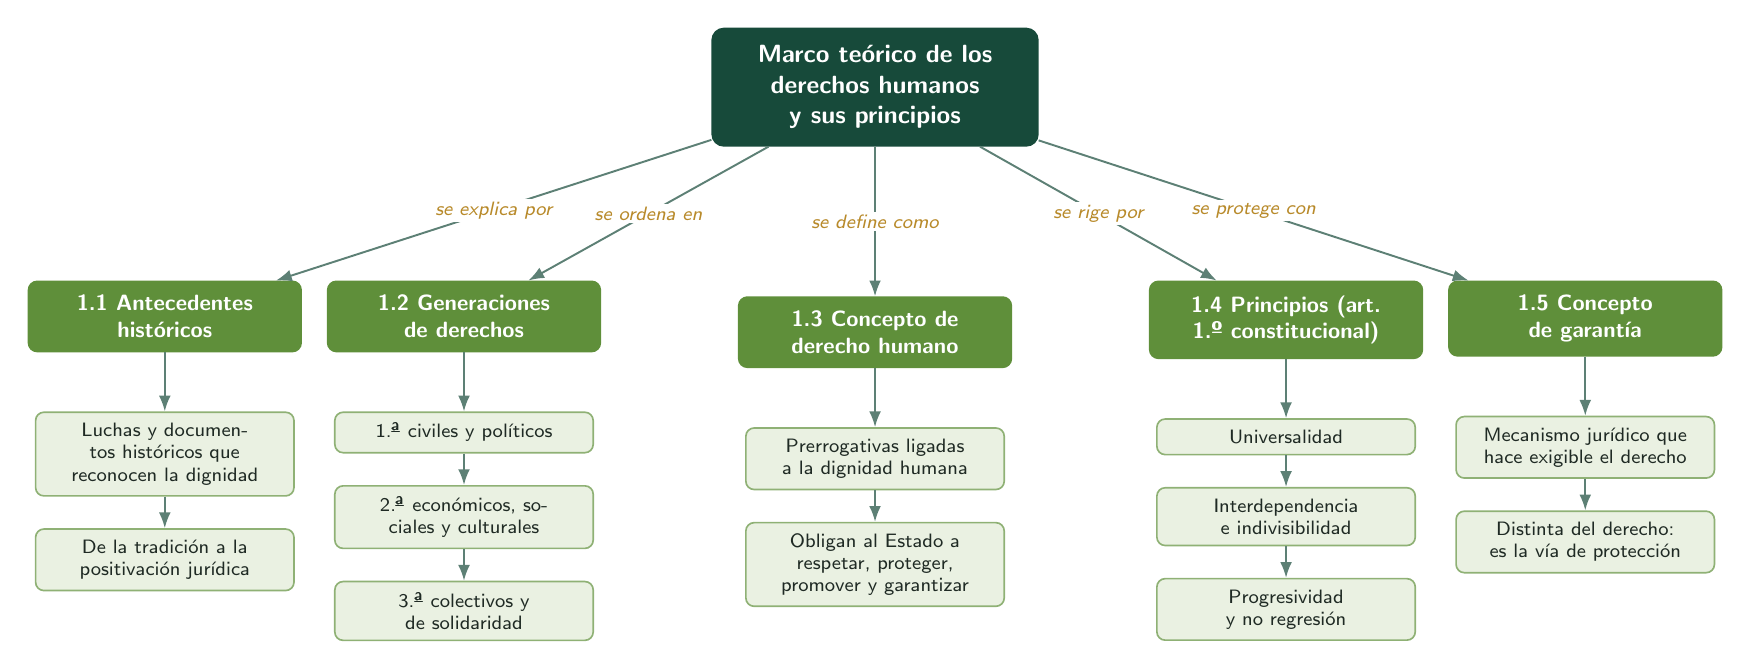
\begin{tikzpicture}[node distance=0.55cm and 0.9cm]

% Nodo raíz
\node[mcroot] (root) {Marco teórico de los derechos humanos y sus principios};

% Ramas de primer nivel
\node[mcbranch, below left=1.7cm and 5.2cm of root] (hist) {1.1 Antecedentes históricos};
\node[mcbranch, below left=1.7cm and 1.4cm of root] (gen) {1.2 Generaciones de derechos};
\node[mcbranch, below=1.9cm of root] (concepto) {1.3 Concepto de derecho humano};
\node[mcbranch, below right=1.7cm and 1.4cm of root] (princ) {1.4 Principios (art. 1.º constitucional)};
\node[mcbranch, below right=1.7cm and 5.2cm of root] (gar) {1.5 Concepto de garantía};

% Enlaces raíz -> ramas
\draw[mclink] (root) -- node[mclabel]{se explica por} (hist);
\draw[mclink] (root) -- node[mclabel]{se ordena en} (gen);
\draw[mclink] (root) -- node[mclabel]{se define como} (concepto);
\draw[mclink] (root) -- node[mclabel]{se rige por} (princ);
\draw[mclink] (root) -- node[mclabel]{se protege con} (gar);

% Hojas: antecedentes
\node[mcleaf, below=0.75cm of hist] (hist1) {Luchas y documentos históricos que reconocen la dignidad};
\node[mcleaf, below=0.4cm of hist1] (hist2) {De la tradición a la positivación jurídica};

% Hojas: generaciones
\node[mcleaf, below=0.75cm of gen] (gen1) {1.ª civiles y políticos};
\node[mcleaf, below=0.4cm of gen1] (gen2) {2.ª económicos, sociales y culturales};
\node[mcleaf, below=0.4cm of gen2] (gen3) {3.ª colectivos y de solidaridad};

% Hojas: concepto
\node[mcleaf, below=0.75cm of concepto] (con1) {Prerrogativas ligadas a la dignidad humana};
\node[mcleaf, below=0.4cm of con1] (con2) {Obligan al Estado a respetar, proteger, promover y garantizar};

% Hojas: principios
\node[mcleaf, below=0.75cm of princ] (pr1) {Universalidad};
\node[mcleaf, below=0.4cm of pr1] (pr2) {Interdependencia e indivisibilidad};
\node[mcleaf, below=0.4cm of pr2] (pr3) {Progresividad y no regresión};

% Hojas: garantías
\node[mcleaf, below=0.75cm of gar] (ga1) {Mecanismo jurídico que hace exigible el derecho};
\node[mcleaf, below=0.4cm of ga1] (ga2) {Distinta del derecho: es la vía de protección};

% Enlaces rama -> hojas
\draw[mclink] (hist) -- (hist1);   \draw[mclink] (hist1) -- (hist2);
\draw[mclink] (gen) -- (gen1);     \draw[mclink] (gen1) -- (gen2);  \draw[mclink] (gen2) -- (gen3);
\draw[mclink] (concepto) -- (con1);\draw[mclink] (con1) -- (con2);
\draw[mclink] (princ) -- (pr1);    \draw[mclink] (pr1) -- (pr2);    \draw[mclink] (pr2) -- (pr3);
\draw[mclink] (gar) -- (ga1);      \draw[mclink] (ga1) -- (ga2);

\end{tikzpicture}

\vspace{0.4cm}
{\footnotesize \textit{Figura 1.} Mapa conceptual del Tema 1. Elaboración propia con base en \citet{alvarezIcazaDerechosMexico}, \citet{rabinovichBerkmanDerechosHumanos} y \citet{marcanoSalazarDerechosHumanos}.}
\end{center}
\end{landscape}

\section{Desarrollo de las ramas del mapa}

\subsection{Antecedentes históricos}

Los derechos humanos no surgen de manera espontánea, sino que son el resultado de un largo proceso histórico de reconocimiento de la dignidad de la persona frente al poder. Rabinovich Berkman muestra que su construcción responde a luchas, conflictos y documentos que, en distintas épocas, fueron ampliando el círculo de personas reconocidas como titulares de derechos y limitando el ejercicio arbitrario del poder \citep{rabinovichBerkmanDerechosHumanos}. Comprender esta dimensión histórica evita una lectura estática: los derechos humanos son una conquista cultural y jurídica que se transforma con el tiempo, y su positivación en constituciones y tratados es una etapa avanzada de ese recorrido.

\subsection{Generaciones de los derechos humanos}

La clasificación por generaciones es una herramienta pedagógica que ordena el desarrollo histórico de los derechos. La primera generación agrupa los derechos civiles y políticos, vinculados con la libertad y la participación; la segunda comprende los derechos económicos, sociales y culturales, orientados a la igualdad material; la tercera reúne los derechos colectivos o de solidaridad, como el medio ambiente sano y la paz \citep{marcanoSalazarDerechosHumanos}. Esta ordenación no implica jerarquía entre generaciones, sino etapas de reconocimiento; de hecho, el principio de indivisibilidad advierte que todos los derechos forman una unidad.

\subsection{Concepto de derecho humano}

El derecho humano es una prerrogativa inherente a la dignidad de la persona, reconocida por el orden jurídico nacional e internacional \citep{alvarezIcazaDerechosMexico}. En el sistema mexicano, el artículo 1.º constitucional establece que todas las autoridades tienen la obligación de promover, respetar, proteger y garantizar los derechos humanos. Esta definición conecta el plano teórico con el plano práctico: no basta con enunciar el derecho, sino que existe un deber estatal correlativo que da sentido a las garantías estudiadas en la asignatura.

\subsection{Principios de los derechos humanos (artículo 1.º constitucional)}

El artículo 1.º constitucional incorpora principios que orientan la interpretación y aplicación de los derechos humanos:

\begin{itemize}
  \item \textbf{Universalidad:} todos los derechos corresponden a todas las personas por su sola condición humana.
  \item \textbf{Interdependencia:} el ejercicio de un derecho suele depender de la realización de otros.
  \item \textbf{Indivisibilidad:} los derechos forman un conjunto que no puede fragmentarse ni jerarquizarse arbitrariamente.
  \item \textbf{Progresividad:} el Estado debe avanzar de forma constante en la protección de los derechos.
  \item \textbf{No regresión:} está prohibido retroceder en el nivel de protección ya alcanzado.
\end{itemize}

Estos principios convierten a los derechos humanos en un marco dinámico y exigible, y son la base para valorar la actuación de las autoridades \citep{alvarezIcazaDerechosMexico}.

\subsection{Concepto de garantía}

La garantía es el mecanismo jurídico que permite hacer efectivo un derecho humano. Conviene distinguir el derecho —el bien o facultad protegida— de la garantía —la vía institucional para exigirlo—. Sin garantías eficaces, los derechos podrían quedar como declaraciones formales sin protección real \citep{marcanoSalazarDerechosHumanos}. Esta distinción es el puente entre el marco teórico del Tema 1 y los medios de control constitucional que se estudiarán posteriormente en la asignatura.

\section{Análisis propio}

La construcción del mapa permite advertir que los cinco ejes del Tema 1 no son bloques aislados, sino una secuencia lógica: la historia explica el origen de los derechos, las generaciones ordenan su desarrollo, el concepto los define, los principios los operativizan y las garantías los hacen exigibles. Mi lectura es que el eje articulador es la distinción entre \textit{derecho} y \textit{garantía}: comprenderla evita el error frecuente de confundir la prerrogativa con el mecanismo que la protege, y prepara el estudio posterior de los medios de control constitucional. En términos de la rúbrica, la síntesis buscó ser jerárquica y concisa sin sacrificar precisión conceptual, priorizando relaciones significativas sobre la mera acumulación de nodos.

\section{Conclusión}

El mapa conceptual del Tema 1 sintetiza el marco teórico de los derechos humanos mostrando cómo sus componentes se articulan en una estructura coherente. Los antecedentes históricos fundamentan su origen; las generaciones ordenan su desarrollo; el concepto los vincula con la dignidad humana; los principios del artículo 1.º constitucional los hacen dinámicos y exigibles, y la noción de garantía introduce la protección efectiva. Mi postura es que este ejercicio de jerarquización no solo cumple una función de estudio, sino que ofrece un mapa mental estable para abordar con mayor claridad los medios de control constitucional, verdadero núcleo de la asignatura de \textit{Garantías Constitucionales}.

\clearpage
\nocite{unadmSitioWeb,cpeum2026,normasApaReferencias2020}
\bibliography{garantias-constitucionales}

\end{document}
